\documentclass{article}

% Please use the following line and do not change the style file.
\usepackage{icml2021_author_response}

% Recommended, but optional, packages for figures and better typesetting:
\usepackage{microtype}
\usepackage{graphicx}
\usepackage{subfigure}
\usepackage{hyperref}       % hyperlinks
\usepackage{booktabs} % for professional tables
\usepackage{amsfonts}       % blackboard math symbols
\usepackage{nicefrac}       % compact symbols for 1/2, etc.

\usepackage{lipsum}

\begin{document}
% Uncomment the following line if you prefer a single-column format
% \onecolumn

First of all we would like to sincerely thank all reviewers for their very detailed and precise remarks on our work. These comments are very useful to improve many aspects of the article, both on theoretical and numerical points.
\begin{figure}[H]
\vskip -0.1in
\begin{center}
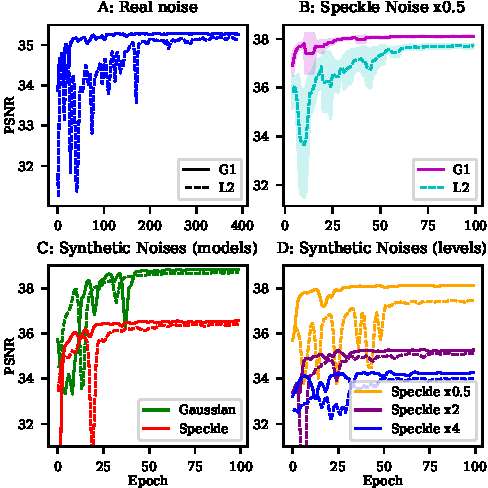
\includegraphics[width=\columnwidth]{fig_review.pdf}
\vskip -0.15in
\caption{PSNR at each epoch on the test set for N-net (G1) or D-net only (L2). A: training on real noise; final performance gain of G1 over L2 is $+0.11dB$. C, D: training on different models/levels of synthetic noise added to ground truth image. C: \textit{Gaussian} and \textit{Speckle} correspond to noises presented in 5.1, that have no and high signal dependency respectively. D: \textit{Speckle} with variance multiplied by 0.5, 2 and 4. B: Mean and SEM over 5 runs.}
\label{fig:review}
\end{center}
\vskip -0.25in
\end{figure}
\paragraph{Contribution of N-net}
We agree that in its original version the several contributions presented in the paper are not properly distinguished.
In the revised manuscript, we propose to highlight the contribution of the N-net to the performance first by adding Fig.~\ref{fig:review}, that show the impact of the N-net on real and several levels of synthetic noise by comparing our model to the D-Net trained with L2 loss (as in N2V, N2S) with every other aspect fixed.
It shows that N-net always improves performances, although not always significantly (this was verified for the 6 datasets considered in the article). Moreover, the addition of the N-net greatly stabilizes the training (see Fig.~\ref{fig:review}B) and improves convergence speed, which enables easier hyperparameters and architecture optimization.
The N-net alone can thus be seen as a modular and \textit{plug-and-play} addition to existing blind denoising models, which always improves performances and convergence.

% explanations:
From the perspective of our framework, the L2 loss can be understood as a particular case of the N-net predicting a constant unit gaussian noise. When the actual noise is significantly different from it (e.g. \textit{Speckle}), the N-net has a stronger impact (see Fig.~\ref{fig:review}C).
From a statistical perspective,  it is known that considering a sufficiently rich noise model is crucial in deconvolution problem to recover the signal distribution (misspecifying the noise density can lead to very poor mean integrated squared error of the deconvolution estimator of the signal distribution).

Moreover the noise model was shown in the paper to capture several statistical behaviors, which is interesting \textit{per-se} and could allow to further improve performances by predicting signal distribution as in (Laine et al. 2019) and PN2V.

\paragraph{Theory}
R2 concerns about the description of loss function indicate that we did not provide enough details to support the proposed loss. It is obtained as an approximation of the negative loglikelihood of the model which will be stated clearly in the revised version as follows.
%The D-net $\mu_\theta(\Omega_y,g(\Omega_y))$ is indeed thought as a model for the expected value of the signal X given the surrounding receptive field excluding the central pixel. This quantity as an estimate of the signal value would indeed minimize the mean squared error to the ground truth and this is what supervised training with MSE does.
The conditional loglikelihood of the observations is written $ \log p(y|\Omega_y) = \log \int p(x,y|\Omega_y) \mathrm{d}x = \log \int p(x|\Omega_y)p(y|\Omega_y,x) \mathrm{d}x$ (*), where $p(y|\Omega_y,x)$ is given by our observation model (1).
As it is very challenging to obtain samples from the distribution $p(x|\Omega_y)$ we propose indeed to estimate this integral by $\log p(y|\Omega_y,\hat {x})$ where $\hat {x}$ is an estimate of $\mathbb{E}[X|\Omega_y]$. Our loss function is then supported by the intuition that $\mu_\theta(\Omega_y,g(\Omega_y))$ is a good approximation of $\mathbb{E}[X|\Omega_y]$. Providing theoretical guarantees that this approximation is good remains an open problem as stated in the original paper. Even though this seems similar to N2V and N2S in terms of loss function we would like to stress that writing explicitly (*) provides a different perspective which we believe:
(1) defines a framework to justify theoretically the proposed approximation (challenging issue); (2) highlights the contribution of $\mu_\theta$ and of the noise model.

\paragraph{Other remarks}
As suggested by R1 and R2, we compared our method to the supervised approach. We chose datasets W2S-1,2 \& 3 where the evaluation dataset is distinct from the training dataset and will include this baseline in the revised manuscript.
We found that our method outperforms the supervised approach of $0.11dB$, $0.22dB$ and $0.26dB$ respectively.
This is not in contradiction with the fact that the central pixel is masked at train time: indeed, our method uses beneficially the central pixel at inference.

% can be removed if necessary
Regarding Noise correlation (R4): only 2 of the 6 datasets display correlation in noise, amplified by the network when not taken into account.
Following (Broaddus et al. 2020) we adapted our masking scheme in that case (see 4.3).

We thank R2 for pointing out erroneous analysis of (Krull et al. 2019). Regarding (Prakash et al. 2020a), it seems that joint learning of noise model was introduced in the pre-print version of March 1st, so after we submitted the manuscript. We will update the manuscript accordingly.

Finally, we emphasize that our method is stable, generic (to types of noises), reproducible (fast and easy code available), so we believe it is a powerful tool for experimenters and a good stepping stone for future research.

% [To be removed si besoin de place] Additionally they model the noise variance as an affine function of the signal intensity. We show that the noise variance may follow a more intricate dependency to the signal intensity and design a more general way to model it
\end{document}
